%!TEX root = ../PhDthesis.tex
\chapter{Modeling the effects of visual statistics on long-range lateral connectivity in visual cortex}

One of the major problems in computational neuroscience is in
understanding how the brain can robustly capture information about its
environment to improve how new information is encoded and
processed. One of the major strengths of developmental models such
as those developed in the previous chapters is that the developed
synaptic connections reflect the visual statistics of the
input. Therefore we can make predictions about how the statistics
embedded in the visual inputs will be reflected in the organization of the
model and could be used to aid cortical computations.

A number of studies have investigated the role visual statistics play
in shaping the organization of cortex. In particular it has been shown
that the distribution of orientations in the orientation maps can be
strongly affected by altering the visual experience of an animal
through manipulations like goggle rearing \citep{Tanaka2006}. However,
the evidence for the encoding of second-order statistics in lateral
connections has been much harder to study, and even coarse approaches
such as measuring the isotropy of lateral connections along the axis
of preferred orientation has not yielded uniform results. While a
number of studies have found that lateral connections are elongated
along the axis of preferred orientation in tree shrew
\citep{Bosking1997}, cat \citep{Schmidt1997}, and owl monkey
\citep{Sincich2001}, in macaque this anisotropy may simply be explained by
the anisotropy in cortical magnification such that the connections are
not actually elongated in visual space \citep{Angelucci2002}.  Whether
the different results reported per species are truly species
differences or simply differences between the various laboratories and
rearing environments involved is not fully clear. Unfortunately, the
tracer injections required to reconstruct the lateral connections can
be performed at most on a few cells in a single animal, making
systematic collection of comprehensive data infeasible.

Although there is a clear lack of data in this area, a few attempts
have been made to go further and establish whether the lateral
projections connect co-circular orientation domains, reflecting the
co-circularity in natural images \citep{Hunt2011}. These studies have
again been inconclusive due to the sparsity of clear data.

In this chapter, we will employ the model introduced in the previous
chapter to analyze to what extent the detailed statistics of the
visual input shape the long-range excitatory connections.  In
particular, we will attempt to reconstruct those statistics based
purely on synaptic weights and the orientation map. In doing so we
will determine to what extent the network has captured the statistics
of the training dataset, and establish whether considerable biases in
the inputs could affect the isotropy of connections.

\section{Methods}

We will first introduce the methods for computing comparable
statistics for natural images and for the LESPI network, which we can
use to analyze how well the network has extracted the underlying
patterns in the training data.

\subsection{Co-occurence statistics}

Natural image statistics have been well characterized in a number of
papers. For instance, \cite{Perrinet2015} analyzed the edge
co-occurence statistics in natural images by labeling images with
edges at varying frequencies, scales, orientations, and phases through
a greedy algorithm, and then computed both the relative orientation
between each pair of edges, and the normalized azimuthal angle between
them. An example image with labeled edges is shown in
Figure~\ref{classifier}, along with a diagram showing how the
co-occurences were computed. Similar analysis approaches have been
used to visualize the co-occurrence statistics in natural images, such
as those produced by \cite{Geisler2001} to predict the performance of
human subjects in contour-detection tasks.

\begin{figure}
	\centering
    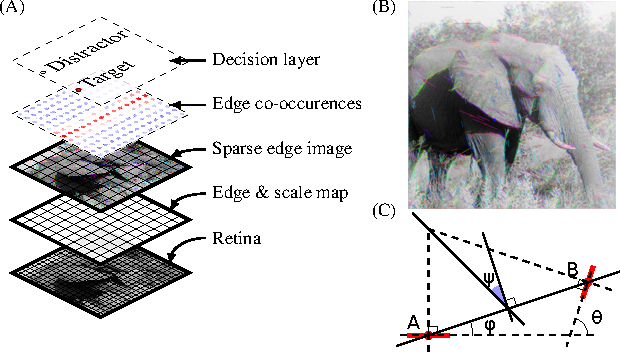
\includegraphics[width=0.8\textwidth]{./classifier.pdf}
	\caption[] {Diagrammatic representation of how a classifier is
      trained to distinguish between outdoor images and inanimate
      objects. A) The different layers used to train the
      classifier. The outdoor images are first fed through a model
      retina, all the edges are labeled with positions and
      scales. Using a greedy algorithm a set of edges accounting for
      the largest amount of luminance variance within the original
      image are selected. Using this set of edges the edge
      co-occurence statistics were computed and finally the classifier
      was trained based on these statistics. B) The sparse set
      of labeled edges extracted from a single image. C) Diagram
      showing how the angular difference $\theta$ and azimuth angle
      $\varphi$ and relative azimuth $\psi$ are computed from two
      edges. Reproduced from \cite{Perrinet2015}.}
	\label{classifier}
\end{figure}

The afferent receptive fields in the visual cortex are usually assumed
to act as feature-selective units. In primary visual cortex,
connections between these neurons could therefore represent the
co-occurence of the features, i.e. second- or higher-order
correlations between simple oriented edges. In order to test this
idea, the models were trained on various synthetic and natural image
datasets, and the statistics embedded in the lateral connections were
decoded.

The geometrical relationship between any pair of neurons each
representing an edge can be defined by three parameters. The
difference in orientation between the two edges $\theta$, computed by
taking the difference in orientation preference between each pair of
neurons. Secondly the distance between the two edges in visual degrees
$d$, computed by calculating the distance between the
center-of-gravity of the weights of each neuron pair. Finally the
angles $\varphi$ and $\psi$, representing the relative and normalized
azimuth between the two edges. The diagram in
Figure~\ref{classifier}C, demonstrates how the angles $\theta$, $\varphi$
and $\psi$ were computed between the edges.

As part of this analysis only post-synaptic neurons with a local
homogeneity index above the 50th percentile, to mirror the procedure
of \cite{Bosking1997} to select only neurons in iso-orientation
domains. As in the previously described analyses the weights were
first thresholded, leaving only the strongest 10\% to ensure that the
model roughly matches the known sparse and patchy pattern observed in
anatomical tracing studies. To compute the preference of the network
for particular arrangements the synaptic weights are combined with the
orientation selectivity of the pre- and post-synaptic neurons and
binned by the three geometric variables described above.

The results of this statistical analysis represents a three
dimensional probability density function based on the synaptic weights
between each arrangement of edges. This data can be binned and
collapsed in a number of ways to evaluate uni-, bi- and multi-variate
relationships that are encoded in the lateral connections.

\subsubsection*{Univariate statistics}

The simplest way to analyze these statistics is to collapse across the
dimensions to visualize the univariate distributions of the $\theta$,
$\varphi$, and distance of connections. This procedure provides (1) an
easily understood analysis to demonstrate how strongly the connections
are biased for similar orientations and co-linear directions, (2) an
indication of how isotropic the lateral connections are in the model,
and finally (3) the distribution of weights by distance.

\subsubsection*{Multi-variate statistics}

Using the computed histogram, various plots can be generated to
compare against the plots produced by directly extracting the edge
co-occurrences from images in the \cite{Perrinet2015} and
\cite{Geisler2001} studies.

\paragraph{Chevron Maps}

The first of these plots (Figure~\ref{SyntheticCooccurrence}), called
a ``chevron map'', presents the bivariate distribution of $\theta$ and
$\psi$, highlighting which spatial arrangement of edges is most likely
to co-occur. In these plots, the central $1^\circ$ diameter region of
the lateral field was ignored so the plot would reflect co-occurrence
statistics of connections \emph{outside} the receptive field of the
neuron. The color in each bin represents the strength of weights for
each arrangement of edges relative to the mean. Therefore dark blue
bins represent edge arrangements that the model learned to be less
likely to co-occur while dark red bins represent arrangements more
likely to co-occur. This procedure also allowed comparing the
co-occurrences between datasets by computing the ratio of normalized
weights in each of the bins, highlighting how the edge co-occurrences
differ between datasets.

\paragraph{Geisler co-occurence plots}

The \cite{Geisler2001} type of co-occurence plots, on the other hand,
reflect three dimensions, the angles $\theta$ and $\varphi$ and the
distance $d$. The plot represents the probability of an edge of a
particular orientation, co-occurring at a particular distance and
azimuth relative to the reference edge. It is then possible to plot
the data to ask two related questions corresponding to the first and
second cooccurrence properties: (1) what is the most likely
orientation difference given a distance and azimuth (i.e.,
$argmax_\theta P(\theta \mid d, \varphi)$), and (2) where is the most
likely position or azimuth of an edge of a specific orientation at a
specific distance (i.e., $argmax_\varphi P(\varphi \mid d,
\theta)$).

While the normalized weights cannot be directly compared to the
relative probabilities obtained by \cite{Geisler2001} through analysis
of various image datasets, they should provide a reasonable proxy for
the co-occurrence probabilities as encoded by the network. Since each
bin represents a circular annulus of different area the weights in
each bin were additionally normalized by their area. In addition to
obtaining the magnitude of the vector sum, a selectivity was also
obtained by dividing the magnitude by the sum of weights. In the final
plots the magnitude is indicated by the color, while the selectivity
at least for the first occurrence property plots is indicated by size.

\subsubsection*{von Mises Model}

Finally, the lateral weights were again fit using the von Mises model
with both Gaussian and orientation-preference--dependent components,
which was first introduced in Section~\ref{BuzasEquations}. This procedure
allows us to provide a quantitative assessment of how well the lateral
connections can be approximated with a simple model that is made up of
orientation, direction, and spatially dependent components. Most
importantly, the direction-dependent component allows us to quantify
how strongly the lateral connection fields are biased along the axis
of preferred orientation, a key issue from the literature.

\subsection{Training stimuli}
\label{synthetic}

Because natural images introduce a variety of RF shapes and phases,
not just long-range correlations, we will first look at the results
from synthetic stimuli constructed to have long-range correlations.
%%
These stimuli are simple extensions of the
elongated 2D Gaussian stimuli used to train the SCAL and SEPI models.
The model will draw 1 pattern per unit area of simulated model, which consists of
a chain of three Gaussian patterns (see
Figure~\ref{GaussianStatistics}). The middle Gaussian determines the
overall orientation ($\theta_M$) of the pattern, and the outer
Gaussians are offset in orientation by a value drawn from a von Mises
distribution with a mean of $\theta_M$ and a $\kappa$ of either $0.5$
or $8$. The patterns are then spatially offset so that they form a
chain forming an `S' shape. By varying the $\kappa$ we can vary how
the distribution of co-occurence statistics affects the preference
for simple elongated bars.

\begin{figure}
	\centering
	\includegraphics[width=1.0\textwidth]{./results/lespi/gaussian_statistics.pdf}
	\caption[Example of Gaussian patterns with co-occurence
      statistics] {Gaussian patterns with co-occurence statistics
      where the orientation offset is drawn from a von Mises
      distribution with different $\kappa$ values changing the
      distribution of orientation offsets.}
    \label{GaussianStatistics}
\end{figure}

We will also train the model on two natural-image datasets that had
previously been analyzed for their co-occurence statistics
(\citealt{Perrinet2015}; see Figure~\ref{classifier}), plus an
additional image dataset recorded in 2010 in juvenile tree-shrew cages
in David Fitzpatrick's lab at Duke University.  The tree-shrew cage
images feature great numbers of highly extended, high-contrast bars
(shown in figure \ref{image_patterns}), and are examples of the
rearing environment for the animals in the \cite{Bosking1997} study.
Thus the statistics of these patterns could be what the
\cite{Bosking1997} tree shrews encoded in their visual cortex, if the
hypotheses from this chapter are valid.

\section{Results}

We will start with the synthetic-stimulus--trained model, to ensure
the approaches work well in the simple case, which we will then extend
to the more complex natural-image--trained models.

\subsection{Synthetic Stimuli}

The stimuli described in Section \ref{synthetic} vary in both relative
orientation and azimuth, which means that if the lateral connections
capture the correlations in the inputs, then these correlations should
also be captured and vary depending on the width of the von Mises
distributions the orientation offsets are drawn from.

\begin{figure}
	\centering
    \includegraphics[width=1.0\textwidth]{./results/lespi/Synthetic_Distributions.pdf}
	\caption[Distributions of lateral connections of models trained on
      synthetic stimuli]{Lateral connections and histograms describing
      their orientation, azimuth and distance dependent distributions
      for narrowly and widely distributed synthetic stimuli. A, B)
      Example lateral excitatory weights after thresholding for the
      widely distributed ($\kappa=0.5$) and narrowly distributed
      ($\kappa=8$) condition. C) Orientation distribution of lateral
      connections, showing stronger bias for iso-orientations in the
      narrowly distributed condition. D) Azimuth distribution, showing
      strong co-linear bias for both conditions. E) Distance
      distribution, showing more weight at distant locations in the
      narrowly distributed condition.}
	\label{SyntheticDistributions}
\end{figure}

By analyzing and binning the lateral weights by orientation
difference, relative azimuth and distance we can get begin to
understand what the lateral connections are actually capturing. The
difference in lateral fields between a model trained on the synthetic
stimuli with a very wide distribution ($\kappa=0.5$) and a much
tighter distribution ($\kappa=8$) is shown in
Figure~\ref{SyntheticDistributions}. These univariate distributions
already demonstrate a clear preference for similar orientations and
co-linear stimuli under both conditions. The histogram of relative
azimuths highlights a strong isotropy along the axis of preferred
orientation. This can indeed be seen even when just looking at the
sample lateral connection fields directly
(Figure~\ref{SyntheticDistributions}A, B). The analysis also
highlights that the model trained on patterns drawn from the tighter
distribution ($\kappa=8$) has a slightly stronger preference for
similar orientations, and more weights at larger distances. This
reflects the stronger bias for long iso-oriented and co-linear
contours in the input patterns.

\begin{figure}
	\centering
        \includegraphics[width=1.0\textwidth]{./results/lespi/Synthetic_Cooccurrences.pdf}
	\caption[Chevron map showing the distribution of orientation and
      azimuth differences between pre- and post-synaptic
      neurons.]{Chevron map showing the distribution of orientation
      and azimuth differences between pre- and post-synaptic neurons
      weighted by connection strength for the wide distribution
      (left), narrow distribution (middle), and the difference between
      them (right). Modeled after the \cite{Perrinet2015}
      co-occurrence analysis of natural images. Each `chevron`
      represents one particular configuration of two edges, varying by
      $\psi$ (relative azimuth) along the x-axis and $\theta$
      (orientation difference) along the y-axis. Increased probability
      is shown in red, and lower probabilities shown in blue. These
      results also highlight that the bias toward similar orientations
      is significantly stronger than for azimuths.}
	\label{SyntheticCooccurrence}
\end{figure}

The chevron map of edge co-occurrences in
Figure~\ref{SyntheticCooccurrence} highlights very similar results. In
particular it demonstrates a greater spread in co-occurring
orientations as the distribution of orientation offsets in the input
pattern widens. Both the azimuth distribution and the co-occurrence
histogram also emphasize an increased preference of parallel alignment
for the tighter distribution. It is not quite clear what drives these
correlations, but through parameter exploration not shown here it was
determined that they could be reduced by presenting fewer overlapping
patterns, suggesting that they were due to increased likelihood of
chance alignments.

\begin{figure}
	\centering
    \includegraphics[width=1.0\textwidth]{./results/lespi/Geisler_Synthetic_Cooccurrence.pdf}
	\caption{Co-occurrence statistics extracted from lateral
      connections to highlight the most likely orientation at each
      distance and azimuth for the two conditions (top row) and the
      most likely azimuth for each orientation and distance (bottom
      row). The colormap represents the relative probability of each
      configuration, while the size reflects the selectivity for that
      particular arrangement. The more narrow distribution ($\kappa$)
      results in more weight at the furthest distances and greater
      confidence in co-circular arrangements, however in both
      conditions co-linearity and co-circularity are decoded almost
      perfectly.}
	\label{SyntheticGeisler}
\end{figure}

The most striking results are obtained by the Geisler-style
co-occurrence histograms in Figure~\ref{SynthethicGeisler}
highlighting how well the network has captured the statistics of the
input and additionally demonstrating how distribution of input
patterns differs with a varying $\kappa$ value. The line segments
shown in the top row of the figure, show, at each of 6 distances and
72 azimuths, the most probable orientation difference. Expressed
differently, for each distance and direction we plotted the preferred
line orientation. The line segments in the bottom row of the figure on
the other hand show, at each distance, the most probable direction for
each possible orientation difference.

In both types of plot we can observe that the same orientation is
encountered along the co-linear axis and as we move away from this
direction the preferred angle slowly shifts away from a parallel to a
co-circular arrangement, which is precisely how the input pattern is
defined. The strength of the co-occurrence probabilities naturally
falls off with distance, and this effect is even stronger in the
$\kappa=0.5$ condition, likely because the distribution is wider and
extended, iso-orientation contours are less likely to occur. This
effect is evident both in the orientation and azimuth co-occurrence
plots.

The top row showing the preferred orientation differences particularly
highlights the increasing preference for extended, co-linear contours
with increasing $\kappa$. The bottom row showing the preferred
direction (or azimuth) on the other hand highlights a slightly greater
spread in azimuths when the distribution of azimuths is wider,
demonstrating that the model can capture differences between the
co-occurence distributions.

\begin{figure}
  \centering
  \includegraphics[width=0.5\textwidth]{./results/lespi/Geisler_Synthetic_Cooccurrence_Diff.pdf
	\caption{The difference in the first co-occurrence property
      between the models trained on synthetic stimuli with flankers
      drawn from a vonMises distributions with $\kappa=8$ and
      $\kappa=0.5$. Shows the ratio between their respective weights
      for each azimuth and weight bin. Underepresentation is
      represented by negative (blue) values, while overrepresentation
      is represented by positive (red) values. This analysis
      highlights the strong overrepresentation of co-linear contours
      at the furthest distances and the slight underrepresentation of
      co-circular edges non-axis aligned azimuths in the $\kappa=8$
      condition when compared to the $\kappa=0.5$ condition.}
	\label{SyntheticGeislerDiff}
\end{figure}

To make the differences even clearer we computed the ratio in weights
for each orientation difference at each distance and direction between
these two conditions and then plotted relative over- and
under-representation of the weights for the $\kappa=8$ compared to the
$\kappa=0.5$ condition. Figure~\ref{SyntheticGeislerDiff} highlights
just how strongly co-linear arrangements are overrepresented in the
$\kappa=8$ condition, with a 20-fold increase in the weight assigned
to this arrangement. The underrepresentation of oblique and orthogonal
arrangements in the $\kappa=8$ condition also reflects the actual
differences between input pattern distribution since a higher $\kappa$
will result in a narrower distribution in the orientation difference
between patterns. This suggest that the network does not only learn a
coarse representation of co-occurrences but also captures more subtle
differences in the input statistics. Having confirmed that the model
can capture such differences for simple, synthetic patterns, we can
extend the analysis to the far greater complexity that is present in
natural images.

\subsection{Natural Images}

Natural and man-made environments have very different statistics,
which may be reflected in the lateral connections in the primary
visual cortex. So far we have seen that the LESPI model can indeed
capture the statistics of a simplified input pattern and distinguish
specific differences in the input statistics. Now we will train the
model on a number of different image datasets, either from outdoor
environments or artificial structures such as laboratory environments
in which animals are raised. Using detailed labeling and analysis of
these datasets, which include those used by \cite{Perrinet2015} and
\cite{Serre2007}, we will demonstrate that the lateral connections in
V1 can already capture the differences between different datasets.  We
will suggest that the rearing environment of an animal can have strong
effects on the organization of the visual system, which should be
considered when using animal models.

Man-made environments are characterized by co-linear, parallel, and
orthogonal arrangements of edges, while true natural images, i.e.,
images of outdoor environments, exhibit more curvature and textured
patterns \citep{Perrinet2015}. In order to test whether the model
would capture these differences, three natural-image datasets were
used: (1) the ``outdoor`` dataset containing a lot of grass textures,
(2) the ``treeshrew`` laboratory cage containing long, high contrast
bars, and (3) the \cite{Serre2007} target dataset of natural scenes
and animals. These represent three highly distinct visual
environments, which should be reflected in long range connections.

\subsubsection*{First-order statistics}

Before investigating more complex second-order statistics, we analyzed
whether particular orientations were hugely overrepresented in the
orientation map, which could introduce systematic biases to the
results. As can be seen in Figure~\ref{NatImgORs}, both datasets show
some bias for specific orientations, with the tree shrew condition
exhibiting a stronger bias along the horizontal and vertical
axes. These biases are likely an artifact arising from the artificial
border at the edge of the simulated sheet, which can affect the whole
map through long-range interactions.

\begin{figure}
	\centering
    \includegraphics[width=1.0\textwidth]{./results/lespi/NatImg_ORDistribution.pdf}
	\caption[Distribution of orientations in the orientation map of
      models trained on outdoor and laboratory images.]{Distribution
      of orientations in the orientation map of models trained on (A)
      outdoor and (B) laboratory images. Although all images were
      rotated to eliminate any inherent biases in the original
      dataset, long-range interactions and border effects still cause
      small biases in the model.}
	\label{NatImgORs}
\end{figure}

\subsubsection*{Second-order histograms}

Once again we compare the isotropy and the orientation and distance
histograms between the two conditions (see
Figure~\ref{NatImgDistributions}), which highlights significant
differences between the datasets. Specifically, the orientation
histogram is biased much more strongly towards iso-orientations in the
outdoor condition. The outdoor condition is also considerably more
orientation selective on average, which is what drives the patchiness
of the lateral connections. However, even though the treeshrew neurons
are much less selective, they actually exhibit a stronger bias along
the axis of preferred orientation, with highly anisotropic lateral
connection fields. Finally, we can see there is much more weight at
distant locations, suggesting the outdoor patterns exhibit more
long-range correlations overall.

\begin{figure}
	\centering
        \includegraphics[width=1.0\textwidth]{./results/lespi/NatImg_Distributions.pdf}
	\caption[Distributions of lateral weights broken down by azimuth,
      orientation, and distance.]{Distributions of lateral weights
      broken down by (A) azimuth, (B) orientation, and (C) distance
      for the outdoor and treeshrew datasets. The treeshrew dataset
      statistics are reflected via much stronger co-linear bias in the
      azimuth histogram even though they are more weakly selective and
      do not extend as far, emphasizing just how strong the co-linear
      bias in the data is.}
	\label{NatImgDistributions}
\end{figure}

\subsubsection*{Chevron Maps}

The chevron maps offer a different view of these effects
(Figure~\ref{NatImgCooccurrences}), as we can now see the relative
co-occurrence along both the relative azimuth and orientation
dimensions, providing an overview of the likelihood of various
geometric arrangements. The views analyzing each dataset individually
highlight once again just how much more biased the connections are
along the $\theta$ dimension, i.e. that the connections are more
biased for similar orientations rather than specific
azimuths. However, the results also demonstrate that in the outdoor
condition co-linear lines are not much more likely than any other
azimuth, which reaffirms the more circular azimuth histogram that can
be seen in Figure~\ref{NatImgDistributions}.

Comparing the distributions to ask whether certain configurations are
more likely in one dataset than the other highlights some more
interesting differences.  Specifically, we can clearly see a stronger
bias for parallel lines in the outdoor dataset and one for orthogonal
lines in the treeshrew dataset. This may reflect the difference
between textured grass patterns with numerous parallel arrangements,
and man-made structures with far more right-angles than would usually
be seen in nature. At the same time, certain curvatures are seen more
strongly in the tree-shrew condition, which is surprising but may
merely reflect the lower orientation selectivity that is evident when
training on that dataset. An analysis that considers the relative
orientation independently from the azimuth may therefore shed more
light on the actual differences.

\begin{figure}
	\centering
        \includegraphics[width=1.0\textwidth]{./results/lespi/NatImg_Cooccurrences.pdf}
	\caption[Chevron map highlighting co-occurrence statistics of
      geometrical arrangements in natural images.]{Chevron map
      highlighting co-occurrence statistics of geometrical
      arrangements in natural images. Red indicates higher probability
      of co-occurrence, while blue indicates lower
      probability. Chevron maps for outdoor and tree-shrew dataset
      shown on top and probability ratios comparing one dataset
      against the other below. Highlights strong bias for co-linear
      and fewer parallel arrangements in the treeshrew dataset, in
      addition to a greater bias towards perpendicular arrangements,
      which are rare in natural images. }
	\label{NatImgCooccurrences}
\end{figure}

\subsubsection*{Co-occurrence properties}

Instead of considering both orientation and azimuth co-occurrences at
the same time, we can treat each separately to ensure that one does
not drown out the other. The first and second co-occurrence property
plots, shown in Figure~\ref{NatImgGeisler} alongside the results from
\cite{Geisler2001} and \cite{Perrinet2015}, make these differences
very clear. Note that while the image analysis performed in these two
studies can directly compute the probability, the model results use
the normalized and weighted synaptic weights as a proxy for the
probability. The magnitude and confidence obtained by computing the
vector sum of the orientation and azimuth co-occurrences are indicated
through color and size respectively.

The right half of Figure~\ref{NatImgGeisler} shows the co-occurrence
of orientation differences obtained from the model and previous
analyses. The results obtained by \cite{Geisler2001} bear out strong
preference for iso-oriented edges, close to and placed along the axis
aligned with the orientation of the reference edge. The results from
the model also show a preference for this arrangment, however there
seems to some distortion in the azimuth for close distances, which may
be caused by imperfect decoding or as a result of the local
interactions that drive column formation. In comparing the direct
image analysis to the model results for the Serre animal dataset and
the tree-shrew--cage dataset, we can make several additional
observations. The tree-shrew data has a stronger bias for parallel and
co-linear edges at almost all azimuths and distances. The animal
dataset on the other hand exhibits more co-circularity in the
orientation differences but has very little preference and selectivity
for arrangements that are orthogonal to the co-linear axis. This
result presumably reflects the fact the treeshrew cages largely
consist of long, parallel lines in form of the bars, while the animal
dataset will contain more smooth, circular contours.

Next we can look at the azimuth co-occurrence preferences (shown on
the left of Figure~\ref{NatImgGeisler}. The results from
\cite{Geisler2001} and \cite{Perrinet2015} indicate some general
patterns, parallel or similarly oriented edges are most likely to
occur along the co-linear and co-circular directions, while oblique
and orthogonal edges mostly occur at angles orthogonal to the
reference edge. The model results also show a similar preference for
the co-occurrence of parallel and similarly oriented edges, but only
the model trained on outdoor images places a number of orthogonal
edges along the axis orthogonal to the reference edge. This suggests
the models is more selective for the azimuth of the co-occuring edge
than its orientation, perhaps reflecting low orientation selectivity.
Looking more specifically at the model trained on the treeshrew
dataset highlights a considerably tighter distribution of azimuth
co-occurrences centered around the co-aligned axis. This suggests that
the treeshrew dataset has more extended, co-linear contours and fewer
co-circular or orthogonal edges when compared to the Serre animal
dataset. While the model results are somewhat noisy this result is
also strongly borne out by the image analysis performed by
\cite{Perrinet2015}, and makes intuitive sense, since the cages are
made up of parallel bars while animals and their environments will
exhibit more co-circularity and criss-crossing textures.


\begin{figure}
  \begin{minipage}[t]{0.6\textwidth}
    \mbox{}\\[-\baselineskip]    \includegraphics[width=\textwidth]{./results/lespi/Geisler_NatImg_Cooccurrence.pdf}
  \end{minipage}\hfill
  \begin{minipage}[t]{0.35\textwidth}
    \mbox{}\\[-\baselineskip]
	\caption{Comparison between co-linearity and co-circularity
      statistics extracted from the model and measured directly from
      the image datasets. Animals and tree-shrew analyses were
      provided by Laurent Perrinet by sparsely labeling edges in the
      image datasets and computing the statistics directly and should
      be directly comparable to the corresponding model
      results. Probability is indicated through the alpha level in the
      animals/tree-shrew analysis, and through color in the Geisler
      and model results. Model results additionally indicate
      confidence through the size of the edge. A number of clear
      conclusions can be drawn. First of all co-linear arrangements
      and extended contours are recognizeable in all datasets. In the
      treeshrew condition the lateral decoding is very confident about
      these arrangements, while in the outdoor conditions similarly
      oriented edges occur at almost all azimuths. Cross-oriented
      edges co-occur with low probability (i.e. strength) but at least
      in the outdoor condition it is confident those do not generally
      occur on the co-aligned axis. Overall this provides strong
      evidence the lateral connections have captured the statistics of
      the input well and although less precise show strong parallels
      to the statistics extracted directly from the images by
      \cite{Geisler2001} and \cite{Perrinet2015} can be seen.}
	\label{NatImgGeisler}
    \end{minipage}
\end{figure}

\subsubsection*{Quantifying the anisotropy}

The analyses so far have allowed us to make qualitative assessments of
how well the lateral connections in the model match the statistics in
the input patterns. In order to test whether the lateral connections
in the model are comparable to the long-range patchy connections in
layer 2/3 of V1 we will also confirm how well the lateral connections
fields are fit by the \cite{Buzas2006} model of lateral connectivity
that was introduced in \ref{BuzasEquations}. By adding the aspect
ratio of the long-range Gaussian as an additional free parameter we
can also quantitatively assess the isotropy along the axis of
preferred orientation to test our hypothesis that the anisotropy of
lateral connections observed in experiments \citep{Bosking1997} could
be explained by differences in rearing environments.

After fitting the model to all the neurons we selected the best fits
for the tree shrew and outdoor conditions and the error between the
fit and the actual weight pattern, allowing us to see features the
model did not capture very well. The comparison between the two fits
is shown in \ref{NatImgvonMises}. It is immediately obvious that the
tree shrew weights are considerably more elongated along the axis of
preferred orientation. The patterns of the error also highlight
several issues, however.  First of all, the fitting procedure seems to
assign too little weight to the nearby iso-orientation patches, which
are strongly connected in the actual weights. There are also patches
that have been assigned weight, yet do not have any in the actual
weight patterns. These are likely associated with phase-inversions,
since the model consists entirely of simple cells, which means that
locally iso-orientation patches with opposite phase are
anti-correlated, a feature the Buzas model does not capture.

\begin{figure}
	\centering
        \includegraphics[width=1.0\textwidth]{./results/lespi/NatImg_vonMises_Fit.pdf}
	\caption[Comparison of \cite{Buzas2006} von Mises model fit
      between the outdoor and treeshrew trained models.]{Comparison of
      \cite{Buzas2006} von Mises model fits between the outdoor and
      tree-shrew--trained models. A, D) Thresholded lateral fields in
      the outdoor and tree-shrew condition. B, E) Model-fitting result
      for the two conditions. C, F) Error between fitted and actual
      lateral weight fields. Overall the patchy organization is
      captured well but the large error at one hypercolumn distance
      suggests the model is not capturing the spatial weight
      distribution perfectly.}
	\label{NatImgvonMises}
\end{figure}

In order to confirm that the model indeed captures the orientation
dependent component well we also let it fit the orientation directly
and confirmed the fitted orientation was well correlated with the
orientation preference in the orientation map. Overall this analysis
showed very high correlation between the estimated and measured
orientation, as can be seen in Figure~\ref{NatImgvonMisesAspect}A We
also plotted the aspect ratio of the long range Gaussian pattern
against the orientation selectivity of the neurons. In the treeshrew
model, the selectivity was highly correlated with the aspect, while in
the outdoor condition this correlation was much weaker. Overall, the
mean aspect ratio for the outdoor condition was 1.29, while the
treeshrew trained model exhibited an aspect ratio of 2.2, suggesting a
much higher anisotropy along the axis of preferred orientation.

\begin{figure}
	\centering
        \includegraphics[width=1.0\textwidth]{./results/lespi/NatImg_vonMises_aspect.pdf}
	\caption[Results from Buzas model fitting.]{Results from Buzas
      model fitting. A) Correspondence between neurons' preferred
      orientations and the orientation estimated based on the lateral
      connection field. B) Dependence between orientation selectivity
      and aspect ratio for the two conditions. Clearly highlights the
      anisotropy in lateral connections trained on the treeshrew
      dataset.}
	\label{NatImgvonMisesAspect}
\end{figure}

\section{Discussion}

In this chapter we explored the effect of changing the co-occurrence
statistics of the visual training on the long-range lateral
connections in a developmental model of V1, in order to test whether
various results concerning the co-circularity \citep{Hunt2011} and
anisotropy of lateral connections \citep{Bosking1997} could be
explained by differences rearing environments. We are also interested
to what extent the early visual cortex is involved in computations
concerning the co-occurrence statistics, to determine whether they
could be involved in computing second or higher-order properties such
as the difference between animal and non-animal objects, which has
been shown to be computed very rapidly in human psychophysics
experiments \citep{Serre2007b}.

In performing the analysis we demonstrated that the model could
capture the statistics of simplified stimuli almost perfectly (see
Figure~\ref{SyntheticGeisler}) and demonstrated that it could even
extract the statistics of far more complex natural-image stimuli to a
reasonable extent, including clear differences between various
datasets. This provides the first demonstration that a developmental
of V1 can indeed capture the statistics of natural images and can
learn various Gestalt rules for edge co-linearity and co-circularity
without hard-coding them. The results suggest that encoding second-
and possibly higher-order statistics in the lateral connections is a
general principle even in the early sensory cortex and predict that
early sensory regions of all modalities should capture these
correlations in some way. The model also makes it clear that the
common assumption that patchy connections in the primary visual cortex
specifically link columns with similar orientation preference is
highly simplistic, with the more interesting story that such
connectivity may simply reflect the co-occurrence probabilities in the
natural world, whatever they may be for a given modality.

Furthermore, we quantify the effect of training the model in a
laboratory environment with very long, high-contrast cage bars, and
suggest that this highly biased rearing environment will have large
implications for the organization of long-range lateral connections.
Specifically, such images exhibit a considerably stronger anisotropy
along the axis of preferred orientation than do outdoor images of
nature.  The tree shrew lateral-connection patterns have an average
anisotropy ratio of 2.2, which is considerably higher than the
anisotropy ratio of 1.29 in the model trained on outdoor images. On
this basis we predict that the large anisotropy ratios observed by
\citep{Bosking1997} may be at least partially explained by the rearing
environment of these animals, which is very different from outdoor
images of nature.

The novel analyses described in this chapter provide a framework to
answer questions about how second-order correlations are captured in
the model. In future, these analyses should be extended to link the
statistics encoded in the lateral connections back to the
surround-modulation effects we previously showed can be mediated by
them. Before such an analysis can be performed, a number of issues
should be addressed.

\subsection{Spatial Frequency}

The spatial frequency distribution of natural images has been well
described in the literature as having a $\frac{1}{f}$
distribution. \cite{Perrinet2015} have shown that the co-occurrence
statistics are generally independent of the spatial
frequency. However, the models in this thesis currently only uses a
single spatial frequency filter at the level of the LGN, meaning that
the other spatial frequencies will be filtered out. The image patterns
in the tree shrew dataset appear to diverge considerably from the
$\frac{1}{f}$ distribution that has been found empirically. Indeed, by
investigating the selectivity of the model trained on tree shrew
images, we could show that they generally have lower spatial frequency
preference than the model trained on the outdoor dataset. This in turn
affects the selectivity of the model, since broader spatial frequency
tuning also results in lower orientation selectivity for a given CF
size. A future analysis should either employ a wider range of spatial
frequency filters at the LGN level or ensure that the distribution of
spatial frequency is approximately equal across the tested datasets.

Such calibration may be particularly important because the orientation
selectivity between the models trained on the treeshrew and outdoor
dataset differs quite considerably, which makes comparing between them
very difficult. The chevron maps in particular are dominated by the
difference in orientation selectivity, which partially obscures the
the differences in azimuths.

\subsection{Complex cells and phase preference}

Another major question regarding the current analysis concerns the
fact that all the modeled neurons are inherently simple cells. As it
is known that long-range patchy connections emerge in layer 2/3, where
there is a mix of simple and complex cells, having only simple cells
in the model makes drawing concrete conclusions very difficult. In
particular, complex cells pool over phase, which means they discard
some of the positional information, complicating the encoding of
relative azimuth between two edges. Extending the model to incorporate
complex cells as outlined in \cite{Antolik2010} may address some of
these questions and would allow us to make concrete predictions about
the differences of lateral connections linking simple and complex
cells, which could be tested in experiments.

Indeed, the large difference in anisotropy that are observed in
tree-shrew lateral connections compared to other species could reflect
the fact that layer 2/3 in tree shrews has a greater proportion of
simple cells, since orientation selectivity is thought to emerge from
the connections between layer 4 and 2/3 rather than thalamocortical
projections as in other species \citep{VanHooser2013}.

\subsection{Local isotropy and suppression}

So far we have mainly discussed to what extent the connections do
reflect the statistics of the natural images the model was trained
on. There are however also clear and systematic differences which
likely reflect properties of the underlying circuit. Since the cortex
has to map high-dimensional visual features onto the 2D surface of the
cortex, there are some tradeoffs in representing all the features
perfectly. In particular, since orientation is mapped onto discrete
columns with other orientations intervening, there is some distortion
in the way position is represented locally.  These distortions can be
seen in some of the co-circularity plots, which show maximal co-linear
enhancement slightly offset from the center. Additionally, the local
isotropic suppression provided by the PV population will strongly
suppress cross-oriented stimuli locally, which means they do not
generally show up in the co-circularity plots as is particularly
evident in the outdoor condition, where they do appear at longer
distances.

From a functional perspective, these do not seem like major issues, if
the lateral connections are primarily concerned with capturing
co-occurrences rather than simply reflecting the preference of the
neuron in the classical receptive field. This issue once again
highlights the importance of considering the visuotopic extent of
lateral connections when compared to the size of the receptive
field. Depending on the species and eccentricity, the neurons could
shift from being primarily devoted to mediating effects within the
classical receptive field to playing a modulatory role in transmitting
information from the extra-classical receptive field. Systematically
characterizing both the receptive field size and the extent of lateral
connections may therefore shed some light on their primary function.

As we concluded in the surround-modulation chapter, the lateral
connections in parafoveal regions of the macaque are just big enough
to mediate interactions at the borders of different textures or
between contour elements and beyond the cRF of a neuron, while more
peripheral regions could integrate larger stimuli.

\subsection{Implications for surround modulation and perception}

Having confirmed that lateral connections can capture the
co-occurrence statistics of the input, it is important to ask what
purpose this may serve. One of the guiding hypothesis of this thesis
and the developmental models on which the thesis is built is that the
mammalian brain self-organizes based on activity-dependent processes
in order to best represent the statistics of the input. This approach
means that identical processes can give rise to the development of
orientation maps in visual cortex and tonotopic maps in the auditory
cortex. Rather than encoding the precise function of each brain
region, the brain robustly yet adaptively organizes in such a way that
it can robustly and accurately encode whatever input it is given. This
idea is supported by experiments performed by the Sur lab, where the
retinal projections to the LGN were rewired to the auditory thalamus.
Sur et al.\ found that animals would develop visual receptive fields
in auditory cortex, and were even able to perform various visual tasks
with no primary visual cortex other than the rewired area
\citep{vonMelchner2000}.

Based on this evidence and the results presented here, we argue that
the organization of the visual cortex is to a large extent an
experience dependent process and even surround-modulation effects such
as contour integration and iso-orientation surround suppression are
emergent phenomena, arising because the cortex learns to represent the
visual statistics of the inputs. The role of lateral connections then
is to learn co-occurrences of the inputs, expressing the model
predictions either as suppressive or facilitatory effects depending of
the geometric arrangement of the stimuli, the contrast and other
contextual information. By learning that edges in the visual
environment are generally co-linearly and co-circularly arranged, even
the very earliest stages of visual processing can contribute towards
complex computations. For instance, such a system could detect
visually salient features through the learned Gestalt grouping laws,
and fill in missing in information based on past experience when the
input is weak or incomplete.

Indeed one of the major findings by \cite{Geisler2001} was the
observation that the local grouping function for contour integration
derived from absolute and Bayesian statistics are very similar. Since
local grouping functions based upon Bayesian statistics are near
optimal, this suggests that learning the absolute co-occurence
statistics may be sufficient to achieve human level performance in
contour grouping. In the analysis of the co-occurrence statistics we
showed that the model was very successful at learning the preferences
for parallel, co-linear and co-circular edge arrangements that are
present in natural images. Future analysis should further explore
whether decoding the neural responses could signal contour groupings,
which could then be compared to the psychophysical results obtained by
\cite{Geisler2001}.

In order to predict to what extent the visual statistics of the
rearing environment affect surround modulation, future
work should focus on generating image patterns from the input
statistics, in order to see how strongly the effects can be modulated
when the statistics either match or clash with the statistics of the
rearing environment. If the statistics play a significant role, then
matching the statistics should maximize the surround-modulation
effects and result in a sparser representation. This property alone
may indeed be sufficient to explain why the responses to natural
images are sparser than those for artificial stimuli.

